\section{Motivación experimental}



\subsection{Modelo de capas}

La hipótesis principal del modelo de capas es suponer que los nucleones se mueven en el núcleo casi independientemente los unos de los otros a pesar de la interacción fuerte. Este movimiento libre significa, en última instancia, que el recorrido libre medio de un nucleón en materia nuclear es grande comparado con las dimensiones del núcleo. En el modelo de capas la interacción nucleón con sus compañeros se reduce a la interacción con un \textbf{campo autoconsciente} (\textit{self-consistent field}) creado por ellos. Generalmente se supone que este campo autoconsciente es estático y esféricamente simétrico.

Debido al corto alcance de las fuerzas nucleares, el potencial del campo autoconsciente tiene dependencia radial muy similiar a la densidad nuclear, es decir, es casi constante dentro del núcleo y se anula fuera. Por lo tanto, en primera aproximación podríamos considerar que el potencial nuclear constante en el interior del núcleo, tal como se hace en el modelo de gas de Fermi ideal\footnote{El modelo de capas incorpora la hipótesis del modelo de gas de Fermi.}, con lo cual las funciones de onda de los nucleones serían ondas planas.

No obstante, cuando introducimos un campo autoconsistente que depende de la distancia al centro del núcleo, las funciones de onda de los nucleones se modifican, a través de la ecuación de Schrödinger, dejando de ser ondas planas. Una vez definido el potencial con el que queramos modelar la interacción nuclear, las soluciones nos llevarán a estados energéticos discretos similares, que como en el caso del átomo de hidrógeno, irá llenando los niveles energéticos de acuerdo con el principio de Pauli. El potencial usado es la suma del potencial de Coulomb, un potencial que contenga la interacción nuclear (el más realista es un potencial de Wood-Saxon), una componente centrífuga y el término de interacción espín-órbita. A través de estos niveles podemos predecir el valor tanto del momento angular total y los posibles estados excitados del núcleo. Existen varias secuencias de llenado de nucleones en la literatura, dependiendo de los parámetros exactos que se usen en la parametrización del campo nuclear autoconsciente. Por ejemplo, usando un potencial nuclear parametrizado como un armónico con término quadrupolar de tal modo que podamos incluir un parámetro que incluya la deformación del núcleo tendríamos una correción del modelo de capas, en el llamado \textit{modelo de Nilsson} \cite{Nilsson:212345}, o por ejemplo el modelo Seniority o BCS \cite{Broglia} que incluye términos de apareamiento. 


En general este es capaz de predecir la mayoría de números mágicos \footnote{Que son ciertos valores de $N$ y $Z$ los núcleos muestran una estabilidad inusual, que se manifiesta, por ejemplo, en una energía de separación de dos nucleones (protones o neutrones) grande.}. Este tipo de modelos funciona muy bien para los núcleos estables, sin embargo no parece predecir correctamente los momentos angulares orbitales y de espín en núcleos exóticos debido a que es necsario incluir más términos en el potencial. Incluir más términos llevará a un reodenamiento de los niveles nucleares que puede cambiar drásticamente las energías de las excitaciones o momentos angulares de las mismas. Precisamente por eso importante estudiar núcleos exóticos, para comparar las predicciones de los modelos nucleares con datos experimentales y así evaluar la validez y las limitaciones del modelo de capas tradicional. Por ello, el estudio de estos sistemas no solo permite entender mejor la estructura nuclear, sino también refinar las herramientas teóricas utilizadas para describirla.

%Por ejemplo, usando un potencial nuclear parametrizado como un armónico con término quadrupolar de tal modo que podamos incluir un parámetro que incluya la deformación del núcleo tendríamos una correción del modelo de capas, en el llamado \textit{modelo de Nilsson} \cite{Nilsson:212345}, o por ejemplo el modelo Seniority o BCS \cite{Broglia} que incluye términos de apareamiento. 



\subsection{Núcleos ricos en neutrones}

Los núcleos ricos en neutrones es uno de los campos de la física nuclear moderna, no solo porque son fundamentales a la hora de entender los procesos r astrofísicos \cite{THIELEMANN2011346}, (proceso de captura rápida de neutrones), los cuales parecen responsables de la creación de la mayor parte de núcleos muy pesados $(60<A)$, que se dan en la expansión tras un colapso del núcleo de una supernova, o la descompresión de la materia neutrónica emitida por la fusion de una estrella binaria compacta de neutrones; sino porque revelan nuevas estructuras nucleares (halos nucleares, modificación del orden de las capas nucleares y números mágicos...). 

Estas nuevas estrucutras nucleares ponen a prueba modelos teóricos y arrojan información necesaria para adaptar modelos fenomenológicos que permitirán obtener resultados teóricos a otros núcleos ricos en neutrones imposibles de medir en experiemntos actualmente por la incapacidad actual de producirlos (debido a su baja estabilidad y su falta de estados ligados). 

La mayor parte de estrucutrasa exóticas la encontramos en la la drip-line, tanto de protones, como de neutrones, sobre la que conocemos únicamente 8 o 9 elementos sobre ella, particularmente en los átomos ligeros. En aquellos que se ha alcanzado esta drip-line los núcleos presentan formas exóticas, comportamientos anómalos que no son vistos en núcleos en la estabilidad. Entre estos comportamientos encontramos los núcleos halo. 

Existen muchas maneras de obtener información acerca la dripline. Por un lado encontramos decaimientos beta, que nos permiten conocer la masa, espín y momentos angulares. Por otro lado las interacciones y secciones eficaces elásticas nos hablan acerca el radio y distribuciones de densidades, las distribuciones a diferentes enerǵias y momentos angulares la presencia de núcleos halo. Las reacciones inelásticas de trasferencia o resonancias elásticas nos pueden arrojar iformación acerca de estados nucleares no ligados \cite{JONSON20041}


\subsection{Núcleo halo}


El halo de neutrones es, en esencia, una manifestación del efecto túnel cuántico, que surge cuando un estado nuclear ligado se encuentra muy próximo al continuo energético \cite{tanihata2023halo}, es decir, a un estado no ligado, y que se entiende como una estrucutra formada por varios cuerpos (uno pesado llamado \textit{core} y varios ligeros) de manera similar a la órbita de un electrón alrededor del núcleo. A los núcleos formados por dos nucleones y un core, tal que el estado con un núcleón y un core es no ligado \cite{tanihata2023lowEnergyHalo} lo llamamos \textbf{núcleo Borremeano}, y podemos encontrar entre ellos $^6$He, $^{11}$Li, $^{14}$Be y $^{17}$B. 



Para que se de una estructura de halo se necesita una combinación de energía de ligadura de neutrones muy pequeña ($<1$ MeV) y una fuerza de corto alcanzce (como es la fuerza nuclear) \cite{tanihata2023halo}, que por ejemplo ene le caso del $^{11}$Li es de $S_{2n}=369.15(65)$ keV \cite{PhysRevLett.101.202501}. El requerimiento de que la energía de ligadura sea pequeña hace que la mayor parte de los halos solo puedan tener uno o dos neutrones en el halo. Dicha combinación de factores permite al neutrón a través del efecto túnel moverse alrededor del core nucleo, lo que conlleva a su vez que el núcleo tenga un tamaño más grande de lo normal: la función de ondas de los neutrones hace probable que este a distancias mucho más lejanas. 

Precisamente esto fue demostrado en 1985 por Tanihata et Al. para el $^{11}$Li, que por aquel entonces era un candidato a ser un núcleo halo. En este experimento hallaron que su radio era un 30\% mayor que el núcleo $^{9}$Li. Teóricamente este estado halo considearba que el core interaccionaba levemente con el núcleo, y que por tanto la distribución de carga debía ser similar entre el litio 9 y el litio 11. Esto fue probado por el ISOLDE, CERN, estudiando el momento cuadrupolar eléctrico \cite{ARNOLD199216} y momento tipolar magnético \cite{Arnold:180144} a través de decaimientos beta. Se había predicho además que la presencia de halos estarían asociadas a grandes secciones eficaces, lo cual también fue demostrado experimentalmente. 


\subsection{Litio 10 y Litio 11}

Como ya hemos dicho, el litio 11 es un núcleo borromeano, para lo cual es condición indispensable que el núcleo litio 10 sea un núcleo no ligado, es decir, que la suma de la masa de los protones y neutrones que la componen sea menor que la masa del propio litio 10. Que sea un estado no ligado implica que solo pueden vivir a través de 

¿Por qué es interesante conocer el estado no ligado litio 10? Por que las función de ondas del $^{11}$Li puede expresarse en realidad como una superposición de diferentes resonancias del $^{10}$Li y un neutrón que ocupa lo que denominamos ``estado orbital relevante'' o último estado orbital (el que define alguna de las características de interés del sistema) \cite{SANETULLAEV2016481}. Además de conocer el estado del litio 10, lo cual puede hacerse a través de varias reacciones, para conocer el litio 11 necesitaremos entender cuales son las relaciones del litio 10 y el neutrón extra.

En principio el litio 10 según el modelo de capas típico debería tener una componente principal de $1p_{1/2}$ tal y como mostramos en \cref{Fig:2-Li10_1}. sin embargo es sabido que debido a la gran cantidad de neutrones que hay en el sistema el modelo de capas habitual no funciona. El reordenamieno producido por el uso de términos adicionales, como puede ser el \textit{modelo de capas de Gamow} llevan a que el estado $2s_{1/2}$ se introduzca entre el $1p_{3/2}$  y el $1p_{1/2}$. 

\begin{minipage}{0.48\linewidth}
    \centering
    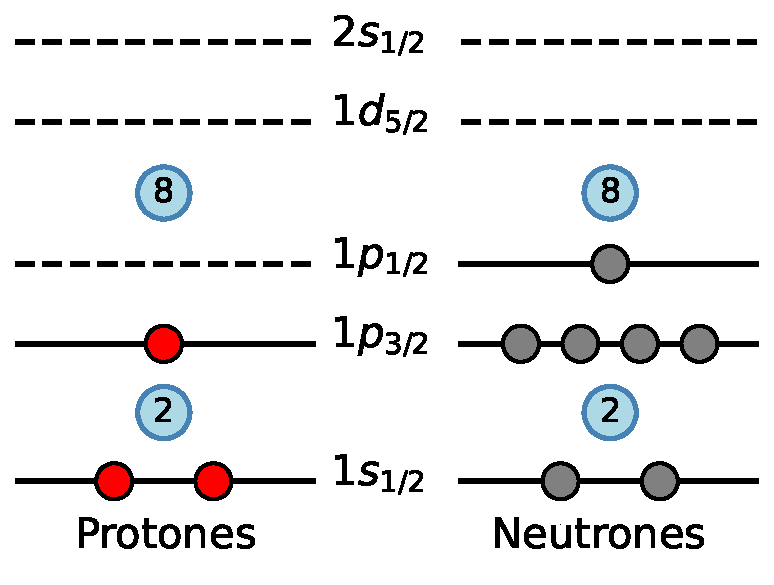
\includegraphics[width=1.0\linewidth]{Imagenes/Capas_10Li.pdf}
    \captionof{figure}{Capas del $^{10}$Li según el modelo de capas tradicional.}
    \label{Fig:2-Li10_1}
\end{minipage}
\hfill
\begin{minipage}{0.48\linewidth}
    \centering
    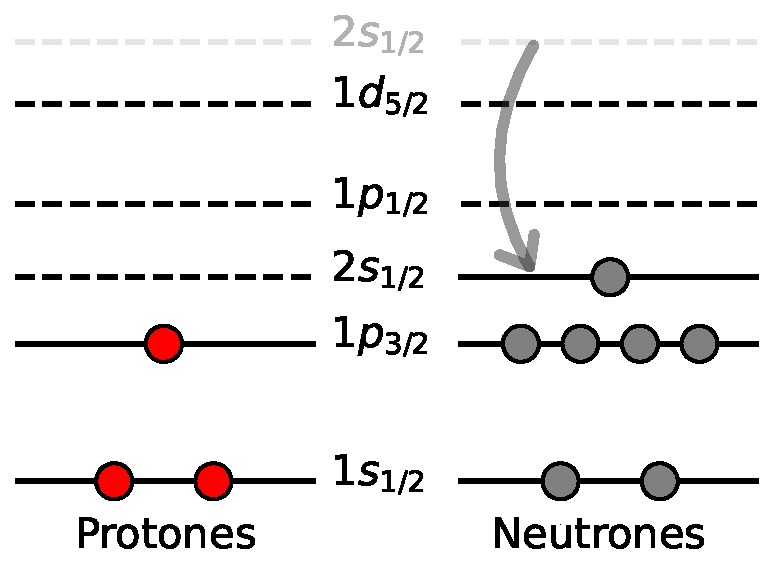
\includegraphics[width=1.0\linewidth]{Imagenes/Capas_10Li2.pdf}
    \captionof{figure}{Capas del $^{11}$Li según el modelo de capas modificado.}
    \label{Fig:2-Li10_2}
\end{minipage}

\vspace*{0.5cm}

Existen diferentes formas de explorar los estados resonantes, siempre a partir de reacciones de trasferencia, como $^{9}\text{Be}(^{9}\text{Be},^{8}\text{B})^{10}\text{Li}$. Diferentes reacciones se pusieron en marcha para poder hallar cual era el estado que dominaba, si el $1p_{1/2}$ o el $2s_{1/2}$, como pueden ser $^{9}\text{Li}(\text{d},\text{p})\text{Li}$ o $^{10}\text{Be}(^{12}\text{C},^{12}\text{N})^{10}\text{Li}$. La mayor parte de estas mostró que efectivamente el primer estado excitado es el $1p_{1/2}$ mientras qeu el estado fundamental era el $2s_{1/2}$. Pese a todo, la mayor parte de las reacciones no estudiaba que grado de influencia tenían estas resonancias en el $^{11}$Li \cite{SANETULLAEV2016481}.

Para esto, la mejor manera de hacerlo es a través de reacciones que quiten neutrones al $^{11}$Li, tal y como pueden ser  $^{11}$Li(p,d)$^{10}$Li o $^{11}$Li(d,t)$^{10}$Li. 




\subsection{Reacción de traferencia $^{11}$Li(d,t)$^{10}$Li}

La reacción en la que nos vamos centrar nosotros es: 

\begin{equation}
   {}^{11}\text{Li} + d \to t + {}^{10}\text{Li}
\end{equation}

Esta reacción es una de las más interesantes a la hora de obtener información acerca de núcleos halo con precisión. Esta es particularmente interesante dentro del estudio del litio 11 debido a su capacidad para proporcionar información directa sobre la estructura halo. A diferencia de muchas reacciones que sólo permiten estudiar el espectro excitado de \({}^{10}\text{Li}\), esta reacción accede directamente a las configuraciones de un solo neutrón en \({}^{11}\text{Li}\), facilitando la reconstrucción de sus componentes estructurales, tal y como hemos mencionado anteriormente.


¿Por qué es relevante estudiar \({}^{11}\text{Li}(d,t){}^{10}\text{Li}\)?
\begin{itemize}
    \item Permite investigar el papel de los estados resonantes de \(^{10}\text{Li}\) en la estructura del halo de \(^{11}\text{Li}\). Dado que $^{10}\text{Li}$ es inestable y no tiene un estado ligado, su estudio experimental es muy complicado, y esta reacción permite observar sus resonancias de forma más directa. \cite{SANETULLAEV2016481}.
    
    \item La transferencia de un neutrón desde \(^{11}\text{Li}\) al deuterón que forma el tritón permite poblar estados de \(^{10}\text{Li}\) con características específicas de momento angular y energía, mostrando la naturaleza de las configuraciones \(s_{1/2}\) y \(p_{1/2}\) en el estado fundamental de \({}^{11}\text{Li}\).  \cite{CASAL2017307}. 
    
    \item Es sensible a los factores espectroscópicos, es decir, permite medir la probabilidad de encontrar una cierta configuración de un neutrón y \({}^{10}\text{Li}\) en el estado fundamental de \({}^{11}\text{Li}\), lo cual no es accesible en muchas otras reacciones. \cite{SANETULLAEV2016481}. 
\end{itemize}

Ventajas frente a otras reacciones de transferencia
\begin{itemize}
    \item A diferencia de otras como \({}^{9}\text{Li}(d,p){}^{10}\text{Li}\), la reacción \({}^{11}\text{Li}(d,t){}^{10}\text{Li}\) accede directamente a la estructura del halo en \({}^{11}\text{Li}\), no sólo a la existencia de resonancias en \({}^{10}\text{Li}\). \cite{CASAL2017307}. 
    
    \item El modelo DWBA aplicado en este tipo de estudios, junto con funciones de solapamiento derivadas de un modelo tridimensional, permite una comparación más directa y realista con datos experimentales. \cite{CASAL2017307}.
\end{itemize}


En resumen, la reacción \({}^{11}\text{Li}(d,t){}^{10}\text{Li}\) no sólo aporta datos sobre los estados de \({}^{10}\text{Li}\), sino que se convierte en una herramienta crucial para entender cómo se configura el halo en \({}^{11}\text{Li}\), permitiendo extraer porcentajes de contribuciones tipo \(s_{1/2}\) y \(p_{1/2}\), y estudiar la ruptura del cierre de capa en \(N=8\). Por ello, tiene una relevancia singular dentro de la física nuclear de sistemas exóticos.

